\documentclass[a4paper,11pt,english]{article}
\usepackage[T1]{fontenc}
\usepackage[utf8]{inputenc}
\usepackage{lmodern}
\usepackage{graphicx}
\usepackage{babel,blindtext}
\usepackage{float}
\usepackage{wrapfig}	
\title{PH21 Assignment 5}
\author{Helen Xue}


\begin{document}

\maketitle


\section{Coin}
\par I used pymc to generate the following plots/distributions, with a chain length of 10k:
\par True probability = 0.4:
\begin{figure}[H]

	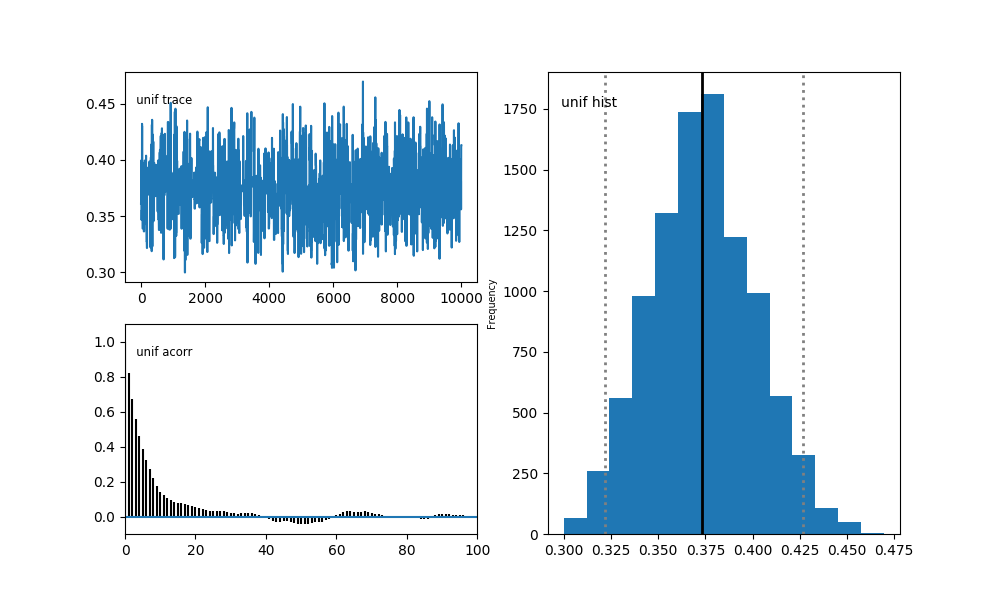
\includegraphics[width=\linewidth]{coin/unif}
	uniform prior coin toss ;   95$\%$ confidence interval: [0.322 0.427]
	
	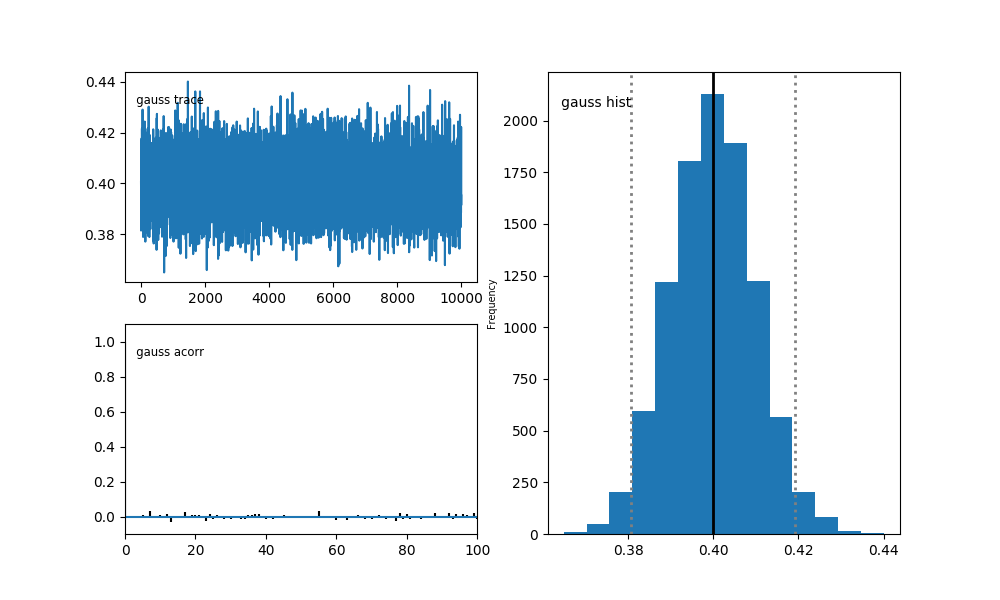
\includegraphics[width=\linewidth]{coin/gauss}
	gaussian prior coin toss ;  95$\%$ confidence interval: [0.395 0.503]
\end{figure}

\par The uniform prior consistently did not converge on the right interval as quickly, even when I increased the chain length to 3000; this is because the uniform prior has more variation.  The trace amplitude is larger, and the peak is less crisp.
\par Varying the bias value for the gaussian prior threw off the results, depending on how much variation we allowed.

\section{Lighthouse}
\par True b = 1.5:
\begin{figure}[H]
	
	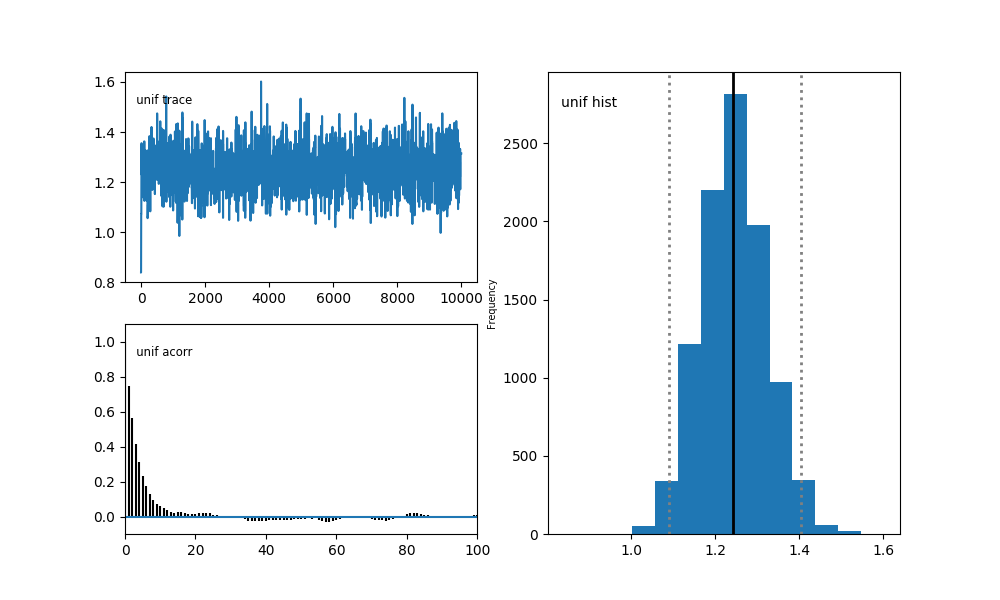
\includegraphics[width=\linewidth]{lighthouse/b_unif}
	uniform prior coin toss ;   95$\%$ confidence interval: [1.186 1.484]
	
	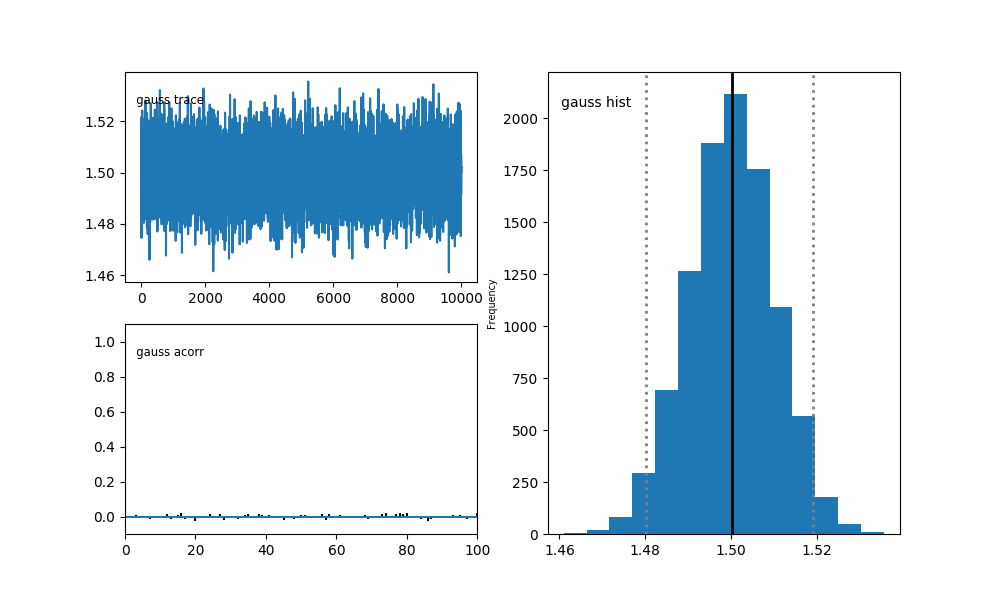
\includegraphics[width=\linewidth]{lighthouse/b_gauss}
	gaussian prior coin toss ;  95$\%$ confidence interval: 
	[1.476 1.513]
	
\end{figure}

\par True a = 1.0:
\begin{figure}[H]
	
	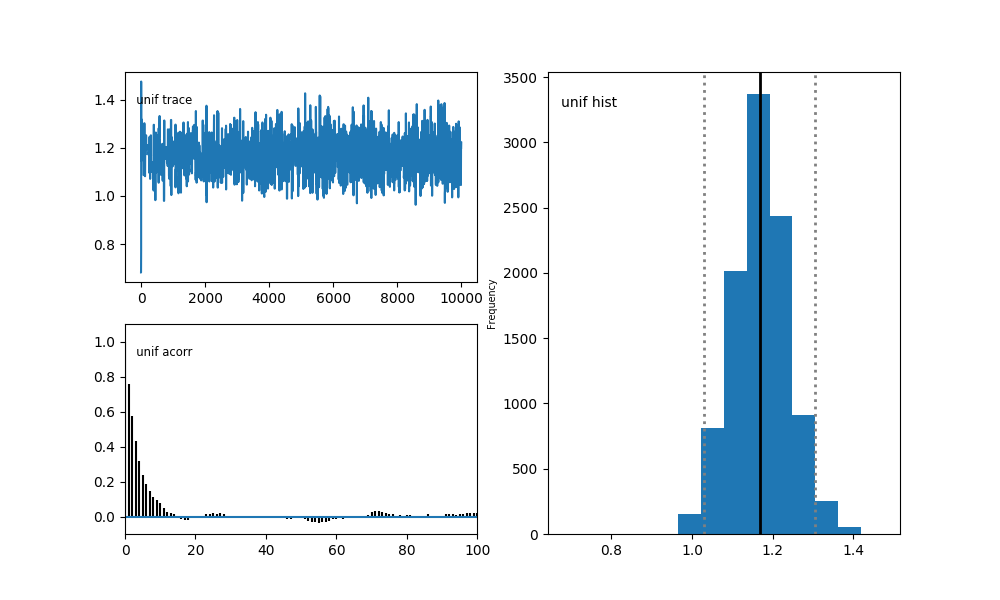
\includegraphics[width=\linewidth]{lighthouse/a_unif}
	uniform prior coin toss ;   95$\%$ confidence interval: [1.134 1.437]
	
		
	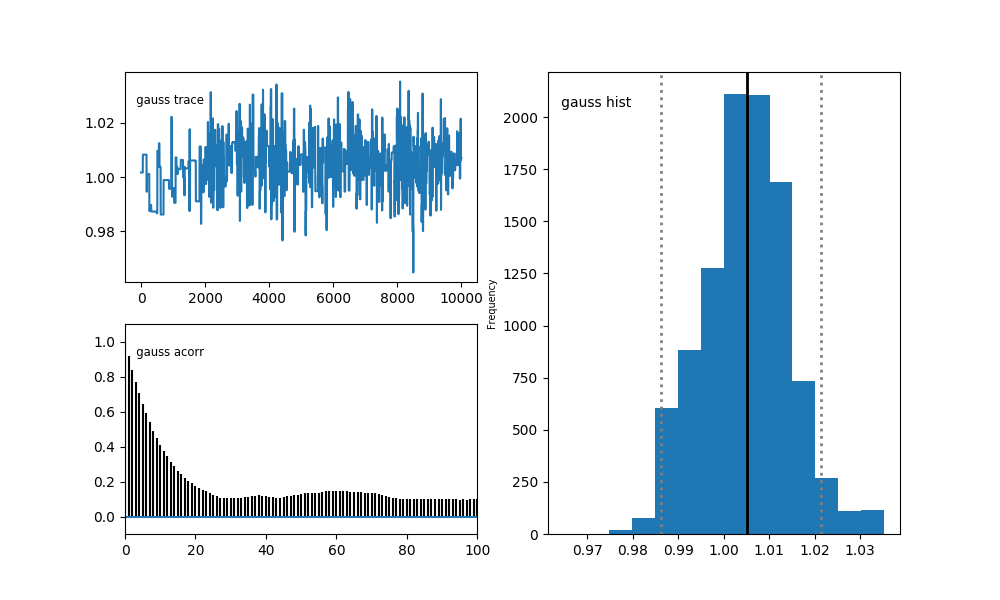
\includegraphics[width=\linewidth]{lighthouse/a_gauss}
	gaussian prior coin toss ;  95$\%$ confidence interval: 
[0.986 1.021]

\end{figure}

\par Similar to before, the uniform prior was consistently less accurate because of its greater variation; here it converged quickly to a wrong mean.
\par The gaussian prior is consistently more accurate.

\end{document}
